\documentclass[a4paper,10pt]{article}
\usepackage[utf8]{inputenc}
\usepackage{xspace}
\usepackage{url}
\usepackage{graphicx,graphics} 
\usepackage{color}
\usepackage{amsmath}
\usepackage{amsfonts}
\usepackage{amssymb}
\usepackage{amsthm}
\usepackage{algorithm}
\usepackage{algorithmic}
\usepackage{longtable}
\usepackage{complexity}
\usepackage{tkz-graph}
\usepackage{float}
\usepackage{setspace}
\renewcommand{\algorithmicrequire}{\textbf{Input:}}
\renewcommand{\algorithmicensure}{\textbf{Output:}}
  
\graphicspath{{figures/}}
\newcommand\rmatching{${\cal R}$-matching\xspace}
\newcommand\mdelay{$\cal M$-delay\xspace}
\newcommand\matchedgraph{{\bf matched graph}}
\newtheorem{proposition}{Proposition}
\newtheorem{theorem}{Theorem}

\setlength{\parskip}{1ex} % Espace entre les paragraphes

\newtheorem{fact}{Fact}
\newtheorem{lemma}[theorem]{Lemma}
\newtheorem{definition}{Definition}
\newtheorem{corollary}{Corollary}



\newcommand{\todo}[1]{{\color{red} TODO: {#1}}}


%opening
\title{Contention Management for 5G}
\author{DB,CC,MG,OM,YS}




\begin{document}

\maketitle
\begin{abstract}
This article treats about Contention Management for 5G.
\end{abstract}
The evolutions proposed in next generations of mobile network architectures aim at evolving toward centralized radio network architectures (C-RAN, for Cloud Radio Access Network) to reduce consumption costs and power at the base stations \cite{mobile2011c}. This type of architecture faces the challenge of mastering the latency in the transfer process between the Remote Radio Heads (RRHs) on the field and baseband units (BBUs) in the cloud. Low latency is already critical for the deployment of C-RAN approach. The standard requires meeting time constraints for functions like HARQ (Hybrid Automatic Repeat reQuest) that needs to be processed in less than from 1 to 10ms \cite{bouguen2012lte}
(depending on targeted services). One specificity in the C-RAN context is not only the latency constraint, but also the periodicity of the data transfer between RRH and BBU (this HARQ constraints must be enforced for each frame emitted every millisecond).\\
 Thus in this article, we work on latency and periodicity constraints in fronthaul.  The best current solution is to rely on an almost full optical approach, where each end-points (RRH on one side, BBU on the other side) are connected through direct fiber or full optical switches \cite{5gppparchitecture}. This architecture is very expensive and hardly scales in the case of a mobile network composed of about 10,000 base stations.  It is then needed to find a solution to offer low latency over commoditized packet based networks. Indeed,  dynamical optical bypass and dynamical management of the emission should be considered to guarantee latency constraints, as it is considered in the french ANR project N-GREEN. This project proposes a new type of switching/routing node and a specific network architecture exploiting WDM packets thanks to a new generation of optical add/drop multiplexers (WSADM: WDM slotted add/drop multiplexer). These packets having a fixed duration close to $1\mu $s are transported in a transparent way, to better exploit the switching matrix of the node; their headers will be transported over one dedicated wavelength at a lower bit rate, to reduce the physical constraints of the electronic processing and scheduler.\\
 Thus, new scheduling and routing paradigms and new technologies have to be considered to  guarantee  delay constrained periodic data transfers. One of the most promising approaches relies on the concept of Deterministic Networking (DN) such that one get rid of
 statistical multiplexing. The traditional queue managements are replaced by time based forwarding. Solutions for Deterministic
 Networking are under standardization in IEEE 802.1 TSN group \cite{finn-detnet-architecture-08}, as well at IETF DetNet working group \cite{ieee802}. Several patents on concepts and mechanisms for DetNet have been already published, see for example \cite{howe2005time,leclerc2016transmission}. To make DN working over a
 network composed of several nodes, it is required to manage the time at which the packets of deterministic paths are crossing each nodes. The major difficulty of this problem is the periodicity of the process. Indeed, a deterministic sending for the messages
between each pair BBU/RRH must not collide with the other messages sent by the others BBU/RRH in the same period, but also in the previous
and following periods.\\

Considering a graph, modeling the network topology, and a set of routes from source nodes (modeling connections to the BBU) and destination nodes (modeling the RRH) in this graph, the purpose is to select, for each destination node a route from one source node to it and a periodic routing scheme allowing to periodically sent a packet to each base station without congestion conflicts between all such packets and to insure a minimum latency. In a slotted time model, the aim is here to minimize the duration of the period, with a constraint of the maximum length of routes to be
selected. Even if the selected set of routes is given this optimization problem has been shown to be  \NP-hard. From an algorithmic point of view,
the purpose of this project is first, to study the complexity and the approximability of this problem when the length of the routes is small
(which corresponds to realistic cases), and secondly, to propose and implement some heuristics to solve this problem on realistic topologies.\\


This problem may look like wormhole problem \cite{cole1996benefit}, very popular few years ago, but here, we want to minimize the time lost in buffers and not just avoid the deadlock, and the wormhole does not treat about the periodicity. Several graph colorings have been introduced to model similar problems such as the allocation of frequencies \cite{borndorfer1998frequency}, bandwidths \cite{erlebach2001complexity}[17] or routes \cite{cole1996benefit}[18] in a network or train schedules \cite{strotmann2007railway}[19]. Unfortunately, they do not take into account the periodicity and the associated problems are also NP-complete. The only model which incorporates some periodicity is the circular coloring \cite{zhou2013multiple, zhu2001circular,zhu2006recent}but is not expressive enough to capture our problem.

\subsection*{Paper organisation}
 In the next section, ...


  

\section{Model}

  \subsection{Definitions}
  

  
	We consider a directed graph $G=(V,A)$ modeling a network. Each arc  $(u,v)$ in $A$ is labeled by an integer $dl(u,v) \geq 1$ that we call the delay and
	which represents the number of time slots taken by a signal to go from $u$ to $v$ using this arc. 
	%Note that for any arc $(u,v)$, $Dl(u,v)=Dl(v,u)$. Dominique voulait être plus général, on mettera cette propriété dans notre topologie
	
      A {\bf route} $r$ in $G$ is a sequence of consecutive arcs $a_0, \ldots , a_{k-1}$, with $a_i=(u_i,u_{i+1}) \in A$. 
      We will often refer to the first element of the route as a source and the last as a target.
      
      The {\bf latency} of a vertex $u_i$ in $r$, with $i \geq 1$, is defined by $$\lambda(u_i,r)= \sum\limits_{0 \leq j <i} dl(a_j)$$ We also define $\lambda(u_0,r)=0$.
      The latency of the route $r$ is defined by $\lambda (r)= \lambda (u_k,r)$.
      

      A {\bf routing function} $\cal R$ in $G$ associates to each pair of vertices $(u,v)$ a route from $u$ to $v$. Let $\cal C$ be an {\bf assignment} in $G$, i.e., a set of couples of different vertices of $G$. We denote by $\cal R_{\cal C}$ the set of routes ${\cal R}(u,v)$ for any $(u,v)$ in $\cal C$. We call $\cal R_{\cal C}$ a {\bf routage graph}, it contains all the informations needed in the forthcoming problems (assignment, routes and delays of the arcs). 
      

      \todo{Si on s'en sert, ajouter ici que le routage est cohérent.}

   \subsection{Slotted time Model}
      Consider now a positive integer $P$ called the {\bf period}. In our problem, we send messages in the network with period $P$. The time will thus be cut into slices of $P$ discrete slots. Assume we send a message at the source $s_i$ of the route $r_{s_i}$, at the time slot $m_{s_i}$ in the first period, then a message will be sent at time slot $m_{s_i}$ at each new period. We define the first time slot at which the message reaches a vertex $v$ in this route by $t(v,r_{s_i}) = m_{s_i} + \lambda(v,r) \mod P$. 

      A message usually cannot be transported in a single time slot. We denote by $\tau$ the number 
      of consecutive slots necessary to transmit a message. Let us call $[t(v,r_{s_i})]_{P,\tau}$ the set of time slots used by $r_{s_i}$ at a vertex $v$ in a period $P$, that is $[t(v,r_{s_i})]_{P,\tau} = \{t(v,r_{s_i}) + k \mod P \mid 0 \leq k < \tau \}$. Usually $P$ and $\tau$ will be clear from the context and we will denote $[t(v,r_{s_i})]_{P,\tau}$ by $[t(v,r_{s_i})]$.
      
      
      A {\bf $(P,\tau)$-periodic affectation} of a routage graph $\cal R_{\cal C}$ is a sequence  ${\cal M}=(m_{s_0}, \ldots ,m_{s_{n-1}})$ of $n$ integers that we call {\bf offsets}, with $n$ the number of routes in $\cal R_{\cal C}$. The number $m_{s_i}$ represents the index of the first slot used in a period  by the route $r_{s_i} \in \cal R_{\cal C}$ at its source $s_i$.
      A $(P,\tau)$-periodic affectation must have no {\bf collision} between two routes in $\cal R_{\cal C}$, that is $\forall (r_{s_i}, r_{s_j}) \in {\cal R_{\cal C}}^2, i \neq j$, % with $\tau$ the size (in number of consecutive slots) of each message that must be periodically sent on each route of ${\cal R}_{\cal C}$, 
      we have $$[t(u,r_{s_i})] \cap [t(u,r_{s_j})] = \emptyset .$$
      

%       Notice that the notion of $P$-periodic affectation \textbf{is not monotone} with regard to $P$. 
      As an example of a $(2,1)$-periodic affectation, let consider a routage graph with routes $\{r_{s_i}\}_{i=0,\dots,n-1}$, such that all pairs of routes intersect at a different edge.
      We set $\tau = 1$ and the delays are chosen so that if $r_{s_i}$ and $r_{s_j}$ have $v$ as first common vertex then we have $\lambda(v,r_{s_i}) - \lambda(v,r_{s_j})=1$.There is a $(2,1)$-periodic affectation by setting all $m_{s_i}$ to $0$.

%       A {\bf conflict graph} represents the collision between the routes of $ {\cal R}_{\cal C}$. The vertices of a conflict graph $G = (V,E)$ are the routes of $ {\cal R}_{\cal C}$, and there is an edge between two vertices if and only if there is a common arc between the two routes in $ {\cal R}_{\cal C}$.
%       
%       Given $u$ and $v$ two vertices of the conflict graph, corresponding to two routes colliding in $ {\cal R}_{\cal C}$. The weight of an edge, $w(u,v)$, is the absolute value of the difference between the distance of the two routes between their respective source node and the collision point.
%       
%       A labeling $F$ of such a graph is an affectation of an integer to each vertex, such that for each vertex $u$, $f(u) \neq f(v)+w(u,v)\mod P$, where $v$ are the neighbors of $u$ in the conflict graph and $P$ our period.
  
      \begin{figure}[ht]
       \begin{center}
      
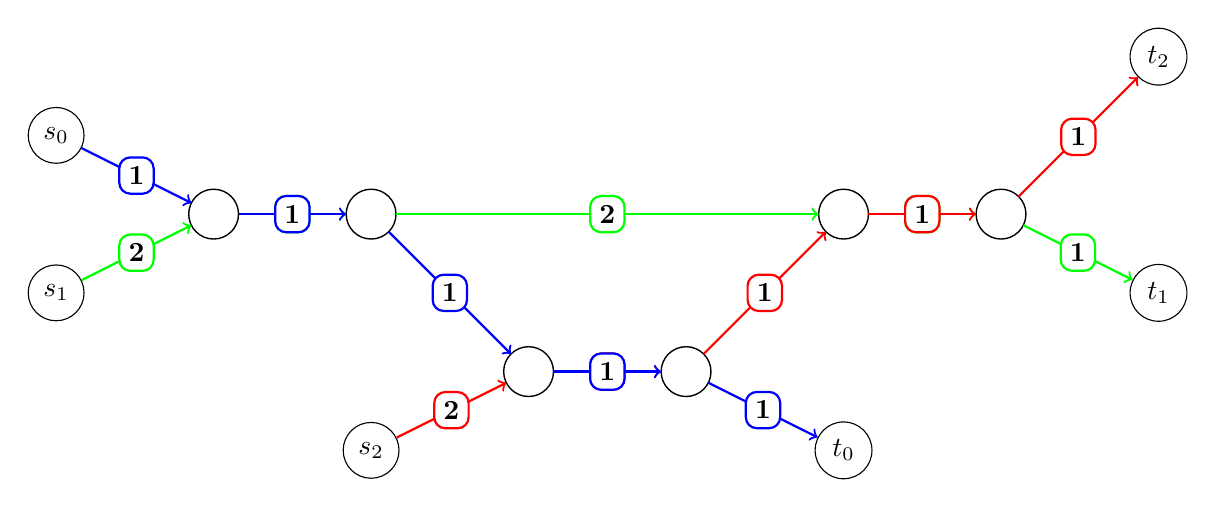
\begin{tikzpicture}


\tikzset{
  LabelStyle/.style = { rectangle, rounded corners, draw,
                       font = \bfseries },
  EdgeStyle/.append style = {->} }
  \SetGraphUnit{5}
  \node[draw,circle] (s3) at (4, 2) {$s_2$}; 
  \node[draw,circle] (s2) at (0, 4) {$s_1$}; 
  \node[draw,circle] (s1) at (0, 6) {$s_0$}; 

  \node[draw,circle] (t3) at (14, 7) {$t_2$}; 
  \node[draw,circle] (t2) at (14, 4) {$t_1$}; 
  \node[draw,circle] (t1) at (10, 2) {$t_0$}; 

  
  \SetVertexNoLabel
  \Vertex[x=2,y=5]{A}
  \Vertex[x=4,y=5]{B}
  \Vertex[x=10,y=5]{C}
  \Vertex[x=12,y=5]{D}
  \Vertex[x=6,y=3]{E}
  \Vertex[x=8,y=3]{F}
  \tikzset{
  EdgeStyle/.append style = {green} }
  \Edge[label = 2](s2)(A)
  \Edge[label = 1](A)(B)
  \Edge[label = 2](B)(C)
  \Edge[label = 1](C)(D)
  \Edge[label = 1](D)(t2)

  
   \tikzset{
  EdgeStyle/.append style = {red} }
  \Edge[label = 2](s3)(E)
  \Edge[label = 1](E)(F)
  \Edge[label = 1](F)(C)
  \Edge[label = 1](C)(D)
  \Edge[label = 1](D)(t3) 
     \tikzset{
  EdgeStyle/.append style = {blue} }
  \Edge[label = 1](s1)(A)
  \Edge[label = 1](A)(B)
  \Edge[label = 1](B)(E)
  \Edge[label = 1](E)(F)
  \Edge[label = 1](F)(t1)

\end{tikzpicture}
      \end{center}
       \caption{A routage graph with $(0,0,0)$ as a $(2,1)$-periodic affectation}
      \end{figure}



   \subsection{Problems}\label{nonmonotone}

    We want to ensure that there is an affectation which allows to send periodic messages from sources to target
    without collisions. The problem we need to solve is thus the following:
    

      \noindent {\bf  Periodic Routes Assignment (PRA)} 

      \noindent {\bf Input:} a routage graph $\cal R_{\cal C}$, an integer $\tau$ and an integer $P$.

      \noindent {\bf Question:} does there exist a $(P,\tau)$-periodic affectation of $\cal R_{\cal C}$ ?


      We will prove in Sec.~\ref{sec:complexity} that the problem PRA is $\NP$-complete, even in restricted settings.
      Even approximating the smallest value of $P$ for which there is a $(P,\tau)$-periodic affectation is hard.

      An unusual property of affectation is that given a routage graph, we may have a $(P,\tau)$-periodic affectation but no
      $(P',\tau)$-periodic affectation with $P' > P$: the existence of an affectation is not monotone with regards to $P$.

	\begin{lemma} \label{lemma:monotonic}
	 For any odd $P$, there is a routage graph such that there is $(2,1)$-periodic affectation but no $(P,1)$-periodic affectation.
	\end{lemma}
\begin{proof}

      Consider the routage graph ${\cal R_{\cal C}}$ given in the previous subsection. 
      We change the delays so that for $v$, the first vertex which belongs to $r_i$ and $r_j$,
      we have $\lambda(v,r_i) - \lambda(v,r_j)= P$, where $P$ is an odd number smaller than $n$, the number of routes in ${\cal R_{\cal C}}$. In such a graph, there is no $(P,\tau)$-periodic affectation, since the problem reduces to finding a $P$-coloring in a complete graph with $n > P$ vertices.\\
      If we consider a period of $2$, for all $i \neq j$, $\lambda(v,r_i) - \lambda(v,r_j) \mod 2 = 1$ . Therefore $(0,\dots,0)$ is a $(2,1)$-periodic affectation of ${\cal R_{\cal C}}$.

      
\end{proof}
      
% 
%       \begin{figure}[H]
%       \label{could-ran}
%       \begin{center}
%       % \begin{tabular}{cc}
%       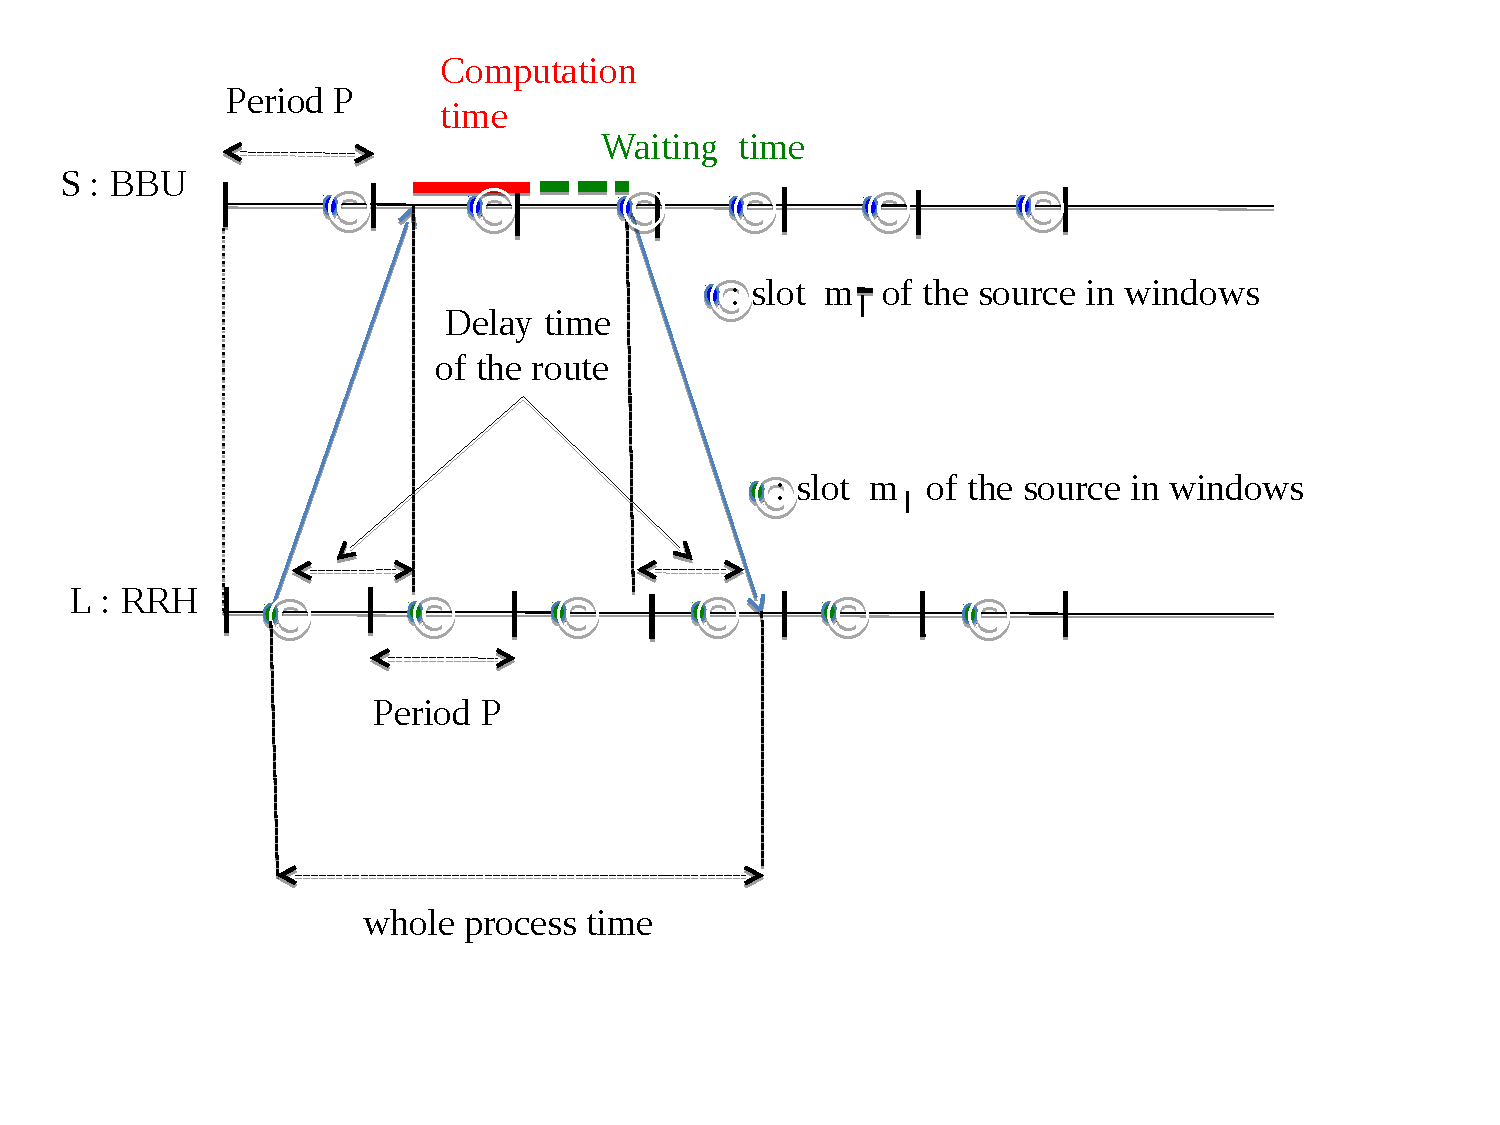
\includegraphics[scale=0.5]{Total-latence.pdf}
%       \caption{Complete process for a leaf in $L$.}
%       \end{center}
%       \end{figure}
%       %\end{tabular}\newline

      
      In the context of cloud-RAN applications, we consider here the digraph $G=(V,A)$ modeling the target network 
      and two disjoint subsets of vertices $S$ and $T$ of equal cardinality, where $S$ is the set of RRHs and $T$ is the set of BBUs. 
      A \textbf{symmetric} assignment ${\cal C}$, is an involutive function from $S$ to $T$, which maps each element $s\in S$ to ${\cal C}(s)$ and ${\cal C}(s)$ to $s$. It can also be seen as the set of pairs $(s,{\cal C}(s))$ and $({\cal C}(s),s)$.\\
      The routing function ${\cal R}$ associates to each couple $(s,{\cal C}(s))$ a route called $r_s$ and to each couples $({\cal C}(s),s)$ a route called $r_{{\cal C}(s)}$.\\     
       We are given a period $P$, a routing function ${\cal R}$, and we consider a $(P,\tau)$-periodic affectation of ${\cal R}_{\cal C}$ which associates $m_s$ to the route $r_s$ which begins by $s$, and $m_{{\cal C}(s)}$ to the routes $r_{{\cal C}(s)}$ which begins by ${\cal C}(s)$.  This affectation represents the following process: first a message is sent at $s$, through the route $r_s$, at time $m_s$.
      
%       
%       We denote by $n$ the size of $S$ and $L$. We are given a period $P$, a routing function ${\cal R}$ and a bijection $\rho:L\rightarrow S$ which assigns a BBU to each RRH. Let ${\cal C}_{\rho} = \{(l,\rho(l))\}_{l \in L} \cup \{(s,\rho^{-1}(s))\}_{s \in S}$. Let consider a $P$-periodic affectation of ${\cal C}_{\rho}$ which associates $m_l$ to 
%       $(l,\rho(l))$ and $m_{\rho(l)}$ to $(\rho(l),l)$.  
      
      
      \begin{center}
      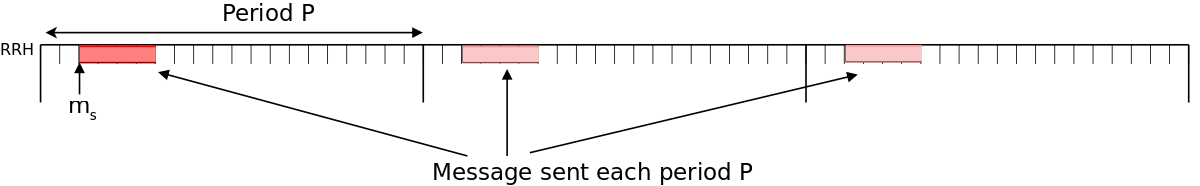
\includegraphics[scale=0.3]{rrh.png}
      \end{center}
      
      

      This message is received by ${\cal C}(s)$ at time $t({\cal C}(s),r_s)$. It is then sent back to $s$ in the same period at time $m_{{\cal C}(s)}$ if $m_{{\cal C}(s)} > t({\cal C}(s),r_s)$, otherwise at time $m_{{\cal C}(s)}$ in the next period. The time between the arrival of the message and the time it is sent back is called the \textbf{waiting time} and is defined by $w_s = m_{{\cal C}(s)} - t({\cal C}(s),r_s)$ if $m_{{\cal C}(s)} > t({\cal C}(s),r_s)$ and $w_s = m_{{\cal C}(s)} + P - t({\cal C}(s),r_s)$ otherwise.
      
       \begin{center}
      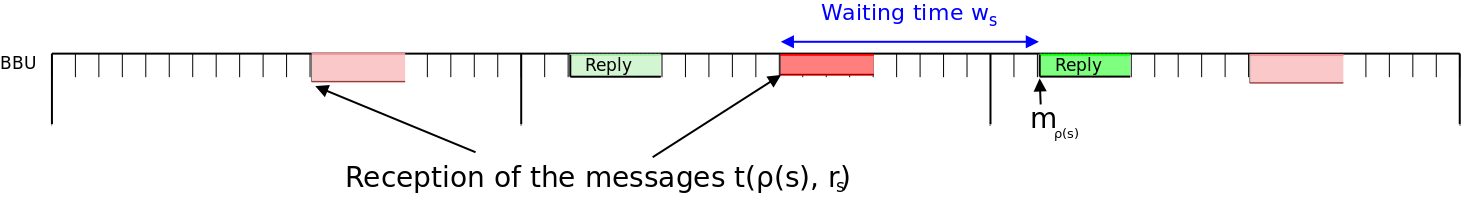
\includegraphics[scale=0.3]{BBU2.png}
      \end{center}
     

      When a BBU receives a message, it must compute the answer before sending it back to the RRH. This time can be encoded
      in the last arc leading to the BBU and thus we need not to consider it explicitly in our model.
    
      Thus, the whole process time for a message sent at vertex $s$ is equal to
      $$
      PT(s)=\lambda(r_s)+ w_s+\lambda(r_{{\cal C}(s)}).
      $$
      
      In the process time, we count the time between the first time at which a message is emitted and 
      the first time at which the message comes back. Alternatively we could consider the time between the emission of the first slot and the reception of the last slot of the message, which would add $\tau$ to the process time.
      However, since all messages are of size $\tau$, it will not change the problem we solve in the rest of the article and that we now introduce.
      
    The {\bf maximum process time} of the $(P,\tau)$-periodic affectation ${\cal M} $ is defined by $MT({\cal M})=\max\limits_{s \in S} PT(s)$. The problem we want to solve is the following. 

      \noindent {\bf Periodic Assignment for Low Latency(PALL)} 

      \noindent {\bf Input:}  A routage graph ${\cal R}_{\cal C}$ with ${\cal C}$ a symmetric assignment, a period $P$, an integer $\tau$, an integer $T_{max}$.

      \noindent {\bf Question:} does there exist a $(P,\tau)$-periodic affectation ${\cal M}$ of ${\cal R}_{\cal C}$ such that $MT({\cal M}) \leq T_{max}$?

      \todo{Si on veut, on peut parler du temps moyen aussi ici, seulement si on fait quelque chose dessus dans la suite}
      %The related optimisation problem we will focus on  consists in minimizing  $MT({\cal M})$. Note that in the context of cloud-RAN networks, we consider $P=1ms$, $\theta=2.6ms$ and $T_{max}$ must be less or equal to $3ms$.
      %cette remarque doit être dans la partie expérimentale



  In this article, we works on a given routage, but we could imagine a problem, in which, considering a given graph $G = (V,A)$ and a period P, the question is to find, if it exists, a routage graph ${\cal R}_{\cal C}$, in which there is $(P,\tau)$-periodic affectation.
  
  
  \todo{Dire si on regle le probleme de trouver un bon routage dans un cas particulier après}
  
  
\section{Solving PRA}
  \label{sec:complexity}
  \subsection{NP-Hardness}

 In this section we assume that the size of a message $\tau$ is equal to one. 
 We will prove the hardness of PRA and PALL for this parameter, which implies the hardness of the general problems. 
Consider an instance of the problem PRA, i.e., a routage graph $\cal{R_{\cal C}}$ and a period $P$. \\
The {\bf conflict depth} of a route is the number of other routes which share an edge with it. 
The conflict depth of a routage graph  $\cal{R_{\cal C}}$ is the maximum of the conflict depth of the routes in $\cal{R_{\cal C}}$.\\
The {\bf load} of a routage graph is the maximal number of routes sharing the same arc.
It is clear that a $(P,1)$-periodic affectation must satisfy that $P$ is larger or equal to the load.


We give two alternate proofs that PRA is $\NP$-complete.
The first proof works already for conflict depth two. Remark that for conflict depth one,
the graph can be seen as a set of disjoint pair of routes, on which PRA and PALL can be solved in linear time. 
 The second proof reduces the problem to graph coloring and implies inapproximability when one tries to find the smallest possible $P$. \\

 \begin{proposition}
Problem PRA is $\NP$-complete, when the routing is of conflict depth two.
\end{proposition}
 \begin{proof}
 The problem $PRA$ is in $\NP$ since given an offset for each route in an affectation, it is easy to check in linear time in the number of edges whether there are collisions.
 
  Let $H=(V,E)$ be a graph and let $d$ be its maximal degree. We consider the problem to determine whether $H$ is edge-colorable
  with $d$ or $d+1$ colors. The edge coloring problem is $\NP$-hard~\cite{holyer1981np} and we reduce it to PRA to prove its $\NP$-hardness. We define from $H$ an instance of PRA as follows. 
  For each $v$ in $V$, the graph $G$ has two vertices $v_1, v_2$, and for each $(u,v) \in E$,the graph G has two vertices $s_{u,v}, t_{u,v}$. Set an arbitrary orientation of the edge $(u,v)$, such that the following route is directed from $u$ to $v$.
  
%   The set $A$ of arcs of $G$ is: 
%   $$ \{(v_1,v_2) \mid v\in V\} \cup \{(u_2,v_1)\mid u \neq v \in V^2\} \cup \{(s_{u,v},u_1),(v_2,t_{u,v}) \mid (u,v) \in E \}. $$
  For each edge $(u,v) \in E$, there is a route $s_{u,v},u_1,u_2,v_1,v_2,t_{u,v}$ in ${\cal R}$.  
  All these arcs are of weight $0$. 
  The set of arcs of G is the union between all the arcs of the previous routes.
  The affectation ${\cal C}$ is the set of pair of vertices $(s_{u,v}, t_{u,v})$.
   
    
  Observe that the existence of a $d$-coloring of $H$ is equivalent to the existence of a $(d,1)$-periodic affectation
  of ${\cal R}_{\cal C}$. Indeed, a $d$-coloring of $H$ can be seen as a labeling of its edges by the integers
  in $\{0,\dots,d-1\}$ and we have a bijection between $d$-colorings of $H$ and offsets of the routes of ${\cal R}_{\cal C}$.
  By construction, the constraint of having no collision between the routes is equivalent to the fact that no two adjacent edges have
  the same color. Therefore we have reduced edge coloring to PRA which concludes the proof. 
 \end{proof}
 \todo{Faire un dessin d'illustration ?}
 
 Remark that we have used zero weight in the proof. If we ask the weights to be strictly positive, which makes sense in our model since
they represent the latency of physical links, it is easy to adapt the proof. We just have to set them so that in any route the delay at $u_1$ is equal to $d$ and thus equal to $0$ modulo $d$. We now lift this hardness result to the problem PALL.

\begin{corollary}
Problem PALL is $\NP$-complete for routing of conflict depth two.
\end{corollary}
\begin{proof}
 We consider $({\cal R}_{\cal C},P,\tau)$ an instance of $PRA$. We assume that no vertex appears both in the first and second position in a pair of ${\cal C}$. Remark that this condition is satisfied in the previous proof, which makes the problem $PRA$ restricted to this kind of instances $\NP$-complete. 
 Let us define $T_{max} = 2 \times \max_{r \in {\cal R}} \lambda(r) + P$. We consider ${\cal C}'$ and ${\cal R}'_{\cal C'}$ symmetrized versions of ${\cal C}$ and  ${\cal R}_{\cal C}$ where for every route there is a symmetric route with new arcs and the same weights.
 The instance $({\cal R'}_{\cal C'},P,\tau,T_{max})$ is in PALL if and only if $({\cal R}_{\cal C},P,\tau)	$
 is in $PRA$. Indeed the waiting time of each route is by definition less than $P$ and thus the maximal process time is always less than $T_{max}$. Moreover a $(P,\tau)$-affectation of ${\cal R}_{\cal C}$ can be extended into a $(P,\tau)$-affectation of ${\cal R'}_{\cal C'}$ in the following way. For each route $r_{u,v}$, the time at which the message arrives is $t(v,r_{u,v})$, then we choose as offset for $r_{v,u}$, $-t(v,r_{u,v}) \mod P$. The symmetry ensures that each new route $r_{v,u}$ in ${\cal R'}_{\cal C'}$ uses the same times slot as $r_{u,v}$ and thus avoid collisions.
\end{proof}

Let MIN-PRA be the problem, given a routage graph and an assignment, to find the minimal period $P$ such that there is a $P$-periodic affectation. 

\begin{theorem}
 The problem MIN-PRA cannot be approximated in polynomial time within a factor $n^{1-o(1)}$, with $n$ the number of routes, unless $\P = \NP$ even when the load is two.
\end{theorem}

\begin{proof}
 We reduce graph coloring to PRA. Let $H$ be a graph instance of the $k$-coloring problem. 
 We define ${\cal R}$ in the following way: for each vertex $v$ in $H$, there is a route $r_v$ in ${\cal R}$.
 Two routes $r_v$ and $r_u$ share an arc if and only if $(u,v)$ is an edge in $H$; this arc is the only one shared by these two routes.   
 All arcs are of delay $0$. 
 
 Observe that the existence of a $k$-coloring of $H$ is equivalent to the existence of a $(k,1)$-periodic affectation in $G$, 
 by converting an offset of a route into a color of a vertex and reciprocally. Therefore if we can approximate the minimum value of $P$ within some factor, we could approximate the minimal number of colors needed to color a graph within the same factor. The proof follows from the hardness of approximability of finding a minimal coloring~\cite{zuckerman2006linear}.
\end{proof}


In particular, this reduction shows that even with small maximal load, the 
minimal period can be large.

    \scalebox{0.5}{

    \begin{tikzpicture}

    \tikzset{
      LabelStyle/.style = { rectangle, rounded corners, draw,
			  font = \bfseries },
      EdgeStyle/.append style = {->} }
      \SetGraphUnit{5}
      
      
      \node[draw,circle] (s3) at (4, 2) {$s_2$}; 
      \node[draw,circle] (s2) at (0, 4) {$s_1$}; 
      \node[draw,circle] (s1) at (0, 6) {$s_0$}; 

      \node[draw,circle] (t3) at (12, 3) {$t_2$}; 
      \node[draw,circle] (t2) at (14, 4) {$t_1$}; 
      \node[draw,circle] (t1) at (10, 2) {$t_0$}; 
      

      \tikzstyle{VertexStyle}=[shape = circle, draw, minimum size = 20pt]
	\tikzset{
      VertexStyle/.append style = {blue} }
	\Vertex[x=-8,y=3]{1}
	      \tikzset{
      VertexStyle/.append style = {green} }
	  \Vertex[x=-7,y=5]{2}

	    \tikzset{
      VertexStyle/.append style = {red} }
	  \Vertex[x=-6,y=4]{3}
		\tikzset{
      VertexStyle/.append style = {black} }
      
      
      \SetVertexNoLabel
      \Vertex[x=2,y=5]{A}
      \Vertex[x=4,y=5]{B}
      \Vertex[x=10,y=5]{C}
      \Vertex[x=12,y=5]{D}
      \Vertex[x=6,y=3]{E}
      \Vertex[x=8,y=3]{F}
      \tikzset{
      EdgeStyle/.append style = {green} }
      \Edge(s2)(A)
      \Edge(A)(B)
      \Edge(B)(C)
      \Edge(C)(D)
      \Edge(D)(t2)

      
      \tikzset{
      EdgeStyle/.append style = {red} }
      \Edge(s3)(E)
      \Edge(E)(F)
      \Edge(F)(t3) 
	\tikzset{
      EdgeStyle/.append style = {blue} }
      \Edge(s1)(A)
      \Edge(A)(B)
      \Edge(B)(E)
      \Edge(E)(F)
      \Edge(F)(t1)
      
	\tikzset{
      EdgeStyle/.append style = {black,-} }

      \Edge(1)(2)
      \Edge(1)(3)
    \node (1) at (-3,4){\Huge $\rightarrow$};
    
    \node (2) at (-7,0){\Huge H};
    \node (3) at (10,0){\Huge G};
    \end{tikzpicture}


    }
    
%     
%   \subsection{Tractable cases of PRA}
%     
%     In this section, we present a few polynomial cases, in particular when the conflict depth is one.
%     When the conflict depth is one, every route can share an arc with only a single other route. 
%     Therefore 
%     
%     
%     The problem PALL seems to be hard to solve, even for very simple classes of graphs, as seen in the next section.
    
\section{The Star Topology}
  
   
    
      In this paper, we consider graphs with a very simple topology that we call the {\bf star topology}. 
      First, for each arc $(u,v)$, there is also an arc $(v,u)$ with the same weight.
      Moreover, there is a special arc, the central arc, which is shared by all routes.
      All routes consist from an arc from its source to the central source node, denoted by {\bf $c_s$},
      then the central arc to {\bf $c_t$}, the central target node, and an arc to its target. In addition to those central nodes, there are two sets of vertices, $S=\{s_0,...,s_{n-1}\}$ and $T=\{t_0,...,t_{n-1}\}$, of cardinality $n$ and ${\cal C}$ a symmetric assignment from $S$ to $T$. 
      The routes are the directed paths of the form $s_i,c_s,c_t,t_i$ and $t_i,c_t,c_s,s_i$. 
      
      
       \begin{center}
	 
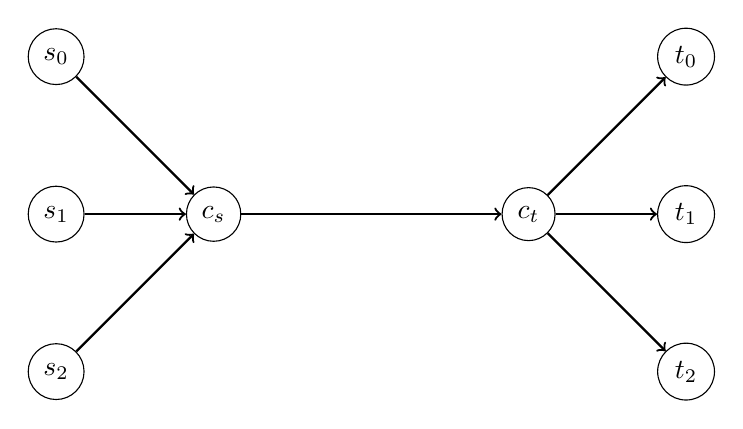
\begin{tikzpicture}

\tikzset{
  LabelStyle/.style = { rectangle, rounded corners, draw,
                       font = \bfseries },
  EdgeStyle/.append style = {->} }

  \SetGraphUnit{5}
  
  \node[draw,circle] (s3) at (0, 0) {$s_2$}; 
  \node[draw,circle] (s2) at (0, 2) {$s_1$}; 
  \node[draw,circle] (s1) at (0, 4) {$s_0$}; 

  \node[draw,circle] (t3) at (8, 0) {$t_2$}; 
  \node[draw,circle] (t2) at (8, 2) {$t_1$}; 
  \node[draw,circle] (t1) at (8, 4) {$t_0$}; 
  

  \node[draw,circle] (cs) at (2, 2) {$c_s$}; 
  \node[draw,circle] (ct) at (6, 2) {$c_t$}; 

  
  \Edge(s1)(cs)
  \Edge(s2)(cs)
  \Edge(s3)(cs)
  
  \Edge(ct)(t1)
  \Edge(ct)(t2)
  \Edge(ct)(t3)
  
  \Edge(cs)(ct)

  
\end{tikzpicture}

  \end{center}
	
      We assume the weight of the central arc to be $0$ since it appears in every route,
      its value does not matter when considering affectations.\\
      Collisions between messages can only appear at node $c_s$ on the way forward and at node $c_t$ on the way back.
      Thus, we only have to check if there is no collisions in a period at those two points.
      We consider two periods P at these vertices, the the {\bf forward period} at $c_s$, and the {\bf backward period} at $c_t$. A message issued by the source $s_1$ at time $m_{s_1}$ will reach $c_s$ at time $m_{s_1} + t(c_s,r_{s_1}) \mod P$ in the forward period, and  $c_t$ at time $m_{t_1} + t(c_t,r_{t_1})\mod P$ in the backward period.

      A $(P,\tau)$-periodic affectation is the choice for all $i < n$, of $m_i$ and $m_{{\cal C}(s_i)}$ such that, for any couple $(j,k)$, we have $[t(c_s,r_{s_{j}})] \cap [t(c_s,r_{s_k})] = \emptyset$ and $[t(c_t,r_{t_j})] \cap [t(c_t,r_{t_k})] = \emptyset$.

      

  \subsection{Solving PALL without waiting times}
  
  In this subsection, we deal with a simpler version of the problem PALL.
  We ask for a $(P,\tau)$-periodic affectation {\bf with all waiting times equal to $0$} and we call this restricted problem {\bf Periodic Assignment for Zero Latency} or PAZL. 
  In that case $MT({\cal M})$ is equal to twice the delay of the longest route, thus $T_{max}$ is not relevant anymore. 
  Since $w_i=0$, choosing $m_i$, the offset of the route from $s_i$ to $t_i$, also sets the offset of the route from $t_i$ to $s_i$ to $m_i + \lambda(r_i) \mod P$.
  Remark that there is a bijection between the affectation of a star topology and the 
  the affectation of the same star topology where all arcs from $s_i$ to $c_s$ have weight equal to $0$
  by changing $m_i$ into $m_i - t(c_s,r_i) \mod P$. Therefore we assume from now on that the \emph{weight of the arcs from $s_i$ to $c_s$ are all equal to $0$}.
  
  \todo{Dire qu'on donne deux algos qui trouvent toujours une solution quand certains condtions sont remplies
  et un dernier qui sait décider si il y a une solution oui ou non mais qui est exponentiel avec des optimisations pour le rendre pratique}
  
    \subsubsection{Shortest-longest policy}
    

    
    We present a simple policy, which works when the period is large with regards to the delay of the routes.
    The message are sent in order from the shortest route to the longest route, without any gap between two messages in the forward period.
    In other words, we assume that the route $r_i$ are sorted by increasing $\lambda(r_i)$ and we set $m_{s_i} = i\tau$.
    We call this algorithm {\bf Shortest-Longest}.
      
     By definition, there are no collision in the forward period and if the period is long enough, 
     it is easy to see that in the backward period the order of the messages are the same as in the forward period and that no collision can occur. 
      
      
      \begin{proposition} When $n\tau + 2(\lambda(r_{s_{n-1}}) - \lambda(r_{s_0})) \leq P$,
      the algorithm Shortest-Longest solves positively PAZL in time $O(n\log(n))$.\label{prop:SL}
      \end{proposition}
      \begin{proof}
       Since $m_{s_i} = i\tau$, $[t(c_s,r_{s_i})] = \{i\tau,\dots, (i+1)\tau -1\}$ and there are no collision on the forward period.
       
       
       We assume may that $\lambda(r_{s_0}) = 0$, since removing $\lambda(r_{s_0})$ to every route does not change the order on the length of the routes and thus the result of this algorithm.
      We have  $[t(c_s,r_{t_i})] = \{2 \lambda(r_{s_i}) + i\tau, \dots,  2 \lambda(r_{s_i}) + (i+1)\tau -1\}$ since $2 \lambda(r_{s_{n-1 }}) + n\tau \leq P$.
       Since $ \lambda(r_{s_i}) \leq  \lambda(r_{s_{i+1}})$ by construction, we have  $2 \lambda(r_{s_i}) + (i+1)\tau -1 < 2 \lambda(r_{s_{i+1}}) + (i+1)\tau$ which proves that there are no collision on the backward period. 
       
       The complexity of the algorithm is dominated by the sorting of the routes. 
      \end{proof}

      
      If the period is slightly smaller that the bound of Proposition~\ref{prop:SL}, a collision will occur on the route in the backward period, making 
      this policy not useful even as a heuristic for longer routes. 

   
    \subsubsection{Greedy Algorithm}
    
    We propose a greedy algorithm to build a $(P,\tau)$-periodic affectation, which provably works when
    the period is large enough with regards to the number of routes and size of messages. In other words, 
    we can always find a solution when the network is far from saturated. 
    
    \begin{proposition}
    Let  $n$ be the number of routes and let $ 3n\tau \leq P$, then there is an algorithm which positively solves PAZL in time $O(n^2)$.
    \end{proposition}
    \begin{proof}
     We consider the forward period and cut it into consecutive interval of size $\tau$ that we call macro-slots. The algorithm works by choosing an offset for each route in the following way: try all offsets which put the message in a yet not used macro-slot in the forward
     period. The choice of an offset also fixes the position of the message in the backward period, chose the first one which does not create a collision. We now prove that this algorithm always finds a $(P,\tau)$-periodic affectation without waiting time when $P \geq 3n\tau$.
     
     Assume we are choosing the offset of the route $r_{k+1}$, we have at least $P - k \geq 3n - k$ free macro-slots in the forward period, since $P \geq 3n\tau$. Each of these $3n - k$ possible offset values translates into $3n - k$ positions of messages in the backward period. All these positions are separated by at least $\tau$ slots. There are already $k$ messages of size $\tau$ in the backward period. One such message can intersect at most $2$ potential positions since they are disjoint intervals. Therefore  amongst the possible $3n - k$ positions, there are  at least $3n - k -2k$ which are without collision. Since $k < n$, $3n - k -2k \geq 1$, which proves that the algorithm terminates and find a  $(P,\tau)$-periodic affectation. 
     
     This algorithm works with a complexity $O(n^2)$, since for the $k^{\text{th}}$ route we have to try at most $2k$ offsets before finding a correct one. We can test the $2k$ offsets of the backward period in time $O(k)$ by maintaining an ordered list of the intervals used by already set routes.
     \end{proof}
     
      \begin{center}
      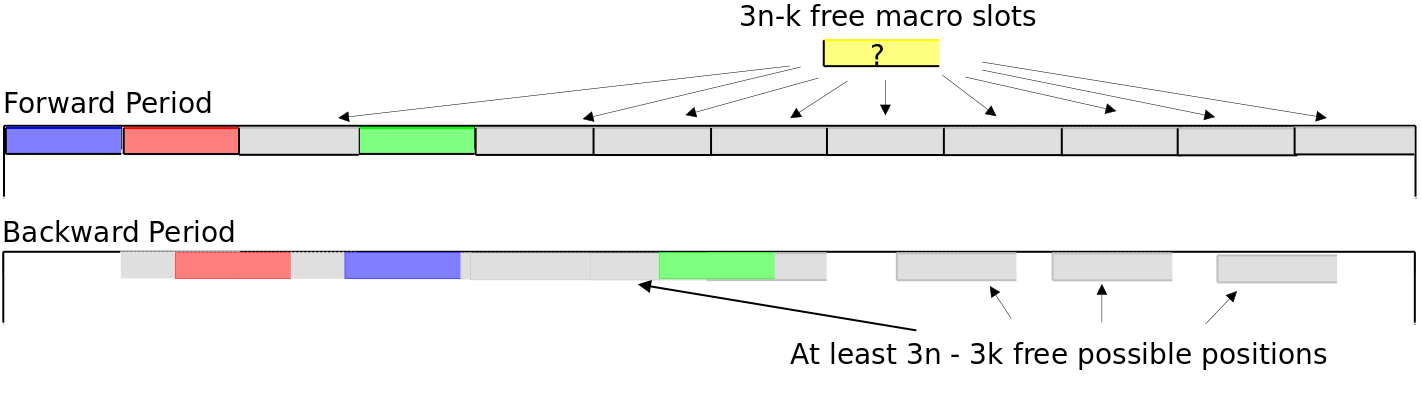
\includegraphics[scale=0.3]{ex3nt.png}
      \end{center}
% 	\begin{algorithm}[H]
% 	\caption{Greedy affectation}
% 	\begin{algorithmic}
% 	\REQUIRE ${\cal R}_{\cal C}$, period $P$
% 	\ENSURE A P-periodic affectation in p $\leq P$, or FAILURE
% 	\STATE $T$ a table of the macro slots of size $\tau$ in the forward period.
% 	\STATE $L$ a list of free intervals in the backward period%$P2[P]$ slots backward period.
% 	\FORALL{source $s$ in S}
% 
% 	\FORALL{free intervals $[a,b]$ in $L$}
% 	\FORALL{ $a/\tau - \lambda(s) <j< b/\tau - \lambda(s)$ }
% 	\IF{ $T[j] == FREE$}
% 	\STATE $m_{s} \leftarrow j.\tau$
% 	\STATE $T[j] = USED$
% 	\STATE update $[a,b]$ in $L$
% 	\STATE BREAK
% 	\ENDIF
% 	\ENDFOR
% 	\ENDFOR
% % 	
% % 	\IF{No intervals are found for $s_i$}
% % 	\STATE return FAILURE
% % 	\ENDIF
% % 	\ENDFOR
% 
% 	\ENDFOR
% 
% 	\end{algorithmic}
% 	\end{algorithm}
	
This algorithm, contrarily to the previous one, may work well, even when the condition $P \geq 3n\tau$ is not true.
In fact, experimental data in Subsection~\ref{sec:experimental_results} suggests that the algorithm works well as soon as $P \geq 1.5 \tau$.

	\subsubsection{Exhaustive search}
% 	\begin{algorithm}[H]
% 	\caption{Exhaustive Generation}  
% 	\begin{algorithmic}
% 	\REQUIRE A routage graph ${\cal R}_{\cal C}$, period $P$, packet size $\tau$
% 	\ENSURE $(P,\tau)$-periodic affectation of ${\cal R}_{\cal C}$
% 	\STATE Forward-budget $\leftarrow$ $P$ - n * $\tau$
% 	\STATE Backward-budget $\leftarrow$ $P$ - n * $\tau$
% 	\STATE Free-Intervals $\leftarrow$ list of free intervals in the backward period, init to $[0;P[$
% 	\FORALL{source $s_i$ in S}
% 	\FORALL{j in Free-Intervals }
% 	\IF{Message of the route $r_{s_i}$ does not collides with scheduled routes}
% 	\STATE $m_{s_i} \leftarrow $ the first slot of Free-Intervals[j]
% 	\STATE Split the Free-Intervals considering the new packet
% 	\STATE Forward-budget $\leftarrow$ Forward-budget - {\em lost size}
% 	\STATE Backward-budget $\leftarrow$ Backward-budget - {\em lost size}
% 	\STATE call Exhaustive Generation on remaining routes
% 	\ENDIF
% 	\ENDFOR
% 	\ENDFOR
% 
% 
%       \end{algorithmic}
%       \end{algorithm}

% 	    
      We now present an exhaustive search algorithm, which tries to set the offsets in all possible ways until it has found a $(P,\tau)$-periodic affectation. Contrarily to the two previous algorithms, when it fails to find a solution, then it certifies there are no solution to PAZL.
      
      We have $n$ routes denoted by $\{0,\dots,n-1\}$. A partial solution $S$ is 
      a partial function from $[n]$ to $\{0,1,\dots,P-\tau -1\}$ which sets a starting time for a subset of the routes $R(S) \subseteq [n]$, such that there are no collisions for these routes.  A partial solution $S'$ extends $S$, if $S'$ is defined over one more route than $S$ and this route has a larger starting offset than all routes of $S$: $R(S') = R(S) \cup \{r'\}$ and for all  $r \in R(S)$, $S(r) + \tau \leq S'{r'}$. We define a tree whose nodes are partial solutions and such that the root is the empty partial solution and 
      the children of a partial solution are the partial solutions which extend it. The solutions to our problem will be the leaves of depth $n$ in the tree, therefore our algorithm is a depth-first search of the tree. 
      
      Remark that a node $S$ with $|R(S)| = k$ can have as many as $(n-k)P$ children. Since the tree is of depth $n$, the tree may have as many as $n!P^n$ elements and while $n$ is small, $P$ may be large which makes its traversal intractable.  Therefore we have to find cuts in the tree to avoid to explore it entirely and henceforth make the algorithm practical. Cuts correspond to the detection of subtrees which contain no solutions and can thus be skipped.   
      We now propose three cuts, the first two being particularly useful when the network is loaded ($n\tau$ is not far from $P$). 
      
      \begin{enumerate}
       \item We consider the number of slots which can be used by routes not yet fixed by a partial solution in the \emph{forward period}. When we extend a solution into $S$ by a route at offset $m$, then at most $(P - m) / \tau $ routes can still be set without collisions in the forward period. If that value is less than the number of routes which are not in $R(S)$, it is a failure and the algorithm backtracks.
       
       \item 
       For the next two cuts, we need to define the notion of the useful slots of a partial solution $S$ in the \emph{backward period}: a slot is said to be useful, if it is not used by a message set by $S$ in the backward period and it belongs to an interval of at least $\tau$ such slots. Useful slots are positions which can be used when extending $S$. We will denote by $([a_i,b_i[)_{i\leq l}$ the ordered sequence of intervals of useful slots of $S$. Without loss of generality we can assume that all $a_i, b_i \leq l$. The number of messages of size $\tau$ which can be placed in the useful slots of $S$ is thus  $\displaystyle{ \sum_{i=0}^{l} (b_{i} -a_i)/\tau } $. If that value is less than the number of routes which are not in $R(S)$, it is a failure and the algorithm backtracks. Notice that the list of intervals of useful slots and the value $\displaystyle{ \sum_{i=0}^{l} (b_{i} -a_i)/\tau } $ can be maintained in constant time, since each time a route is added, we only need to split an interval of useful slots into at most two such intervals.
       
       
       \item 
       Let $S_1$ and $S_2$ be two partial solutions with $R(S_1) = R(S_2)$. Let $US_1$ (respectively $US_2$) be the set of useful slots of $S_1$ (resp. $S_2$). We say that \emph{$S_1$ dominates $S_2$} if there are more useful slots both in the forward and backward periods for $S_1$ than for $S_2$. Formally, the largest offset fixed in $S_1$ is smaller than the one in $S_2$ and $US_2 \subseteq US_1$. Remark that any valid sequence of extensions of $S_2$ (choosing offsets of routes in the complementary of $R(S_2)$) is also a valid sequence of extensions of $S_1$. Therefore if the tree rooted at $S_2$ contain a solution, then $S_1$ contains one too. Hence, in our exhaustive search of the tree of partial solutions, we can skip the tree rooted at $S_2$.
       
       We now explain how we can detect some partial solutions which are dominated so that we do not explore their subtrees.
       Consider a partial solution $S$ which we extend into $S'$ by setting the offset of the route $r$ to be the smallest possible. The offset of $r$ in the backward period is $S'(r)+ \lambda$ and we denote the end of the message before before by $a$. Hence all extensions of $S$ into $S''$ such that $S'(r)  < S''(r) < a + \tau - \lambda$ are dominated by $S'$. Therefore when computing the extension of $S$, we first build $S'$ and then $S''$ with $S''(r) =  a + \tau - \lambda$ , skipping all values in between.
       
             \end{enumerate}
      
      The third cut works well in conjunction with the first one since it makes the offsets grow quickly and 
      which makes the first cut more likely to apply. A last cut could be implemented: compute for every route not in $R(S)$ the set of possible positions in the backward period and verify whether at least one is contained in the useful slots of $S$.


    \subsubsection{Experimental Results}\label{sec:experimental_results}
      
      The following experimental results help compare the three presented algorithms.
      Notice that both Greedy algorithm and the Shortest-Longest are polynomial time algorithm but are not always able to find a solution. On the other hand, the exhaustive search will find an optimal solution, if it exists, but works in exponential time. We will compare the performance of the algorithms in two different regimes: the routes are either short with regards to $\tau$ and $P$ or unrestricted.
      We choose the parameter realistic with regard to our C-RAN context. The number of routes 
      is at most $n = 20$, $\tau$ is equal to $2500$ and the period is at most $3n\tau$ (otherwise the greedy algorithm always returns a solution). 
      
      \todo{Dire où on peut trouver le code (pas la peine de donner des infos sur la machine/compilateur car one ne fait pas d'étude de performances.}
%             
%             The graphs 
%       To correspond with the C-RAN applications, we made some simulations on graphs in which $\lambda(c_s,r_{s_i})$ and $\lambda(c_t,r_{t_i})$, are drawn following an uniform act between 0 and 700 slots, that is, at the most, 5 km between the RRH and its BBU. The messages size $\tau$ is to 2500 slots, that is, approximately 1.228 Gbps of data for each route. The size of a slot is given by the time taken to send 64 bytes on the network, in which the links has 10Gbps throughput.
% 
%       \todo{Mettre les données concrètes plus proprement et éventuellement ne pas les mettre si on envoie pas à un truc de télécom}

      \paragraph{Short routes}
      
      First we consider routes which are shorter than $\tau$, that is a message cannot be contained 
      completely in a single edge. This is typical in our context and we will consider graphs in which the values $\lambda(c_t,r_{t_i})$ are drawn uniformly between $0$ and $700$ slots. It corresponds to messages of size blah and links of bandwidth 10Gbps and length less than blah. 
      
      \todo{à compléter}
      
      Our aim is to understand how well the algorithms are working when the network has a high load (when 
      the load is low, the greedy algorithm always returns a solution). To do that we try to evaluate the 
      minimal period for which a $(P,\tau)$ periodic affectation can be found by each algorithm. 
      To that end we do a linear search on $P$, since a dichotomy would not work because of Lemma~\ref{lemma:monotonic}.
      
      
      In our experiment, we generated $1000$ random instances of PAZL for $1$ to $12$ routes. 
      We measured the average minimal period, for each algorithm. We needed to stop our experiments at $12$ routes since the exhaustive search was taking more than a second to finish on many instances.
      Note that the exhaustive search is optimal, that is it finds the best possible period for a given instance. 
      We also drew the function $f(n) = n\tau$, which is an absolute lower bound on the period and $g(n) = 3n\tau$ which is the theoretical upper bound of the greedy algorithm.
      
      
        
        \begin{figure}

      \begin{center}
      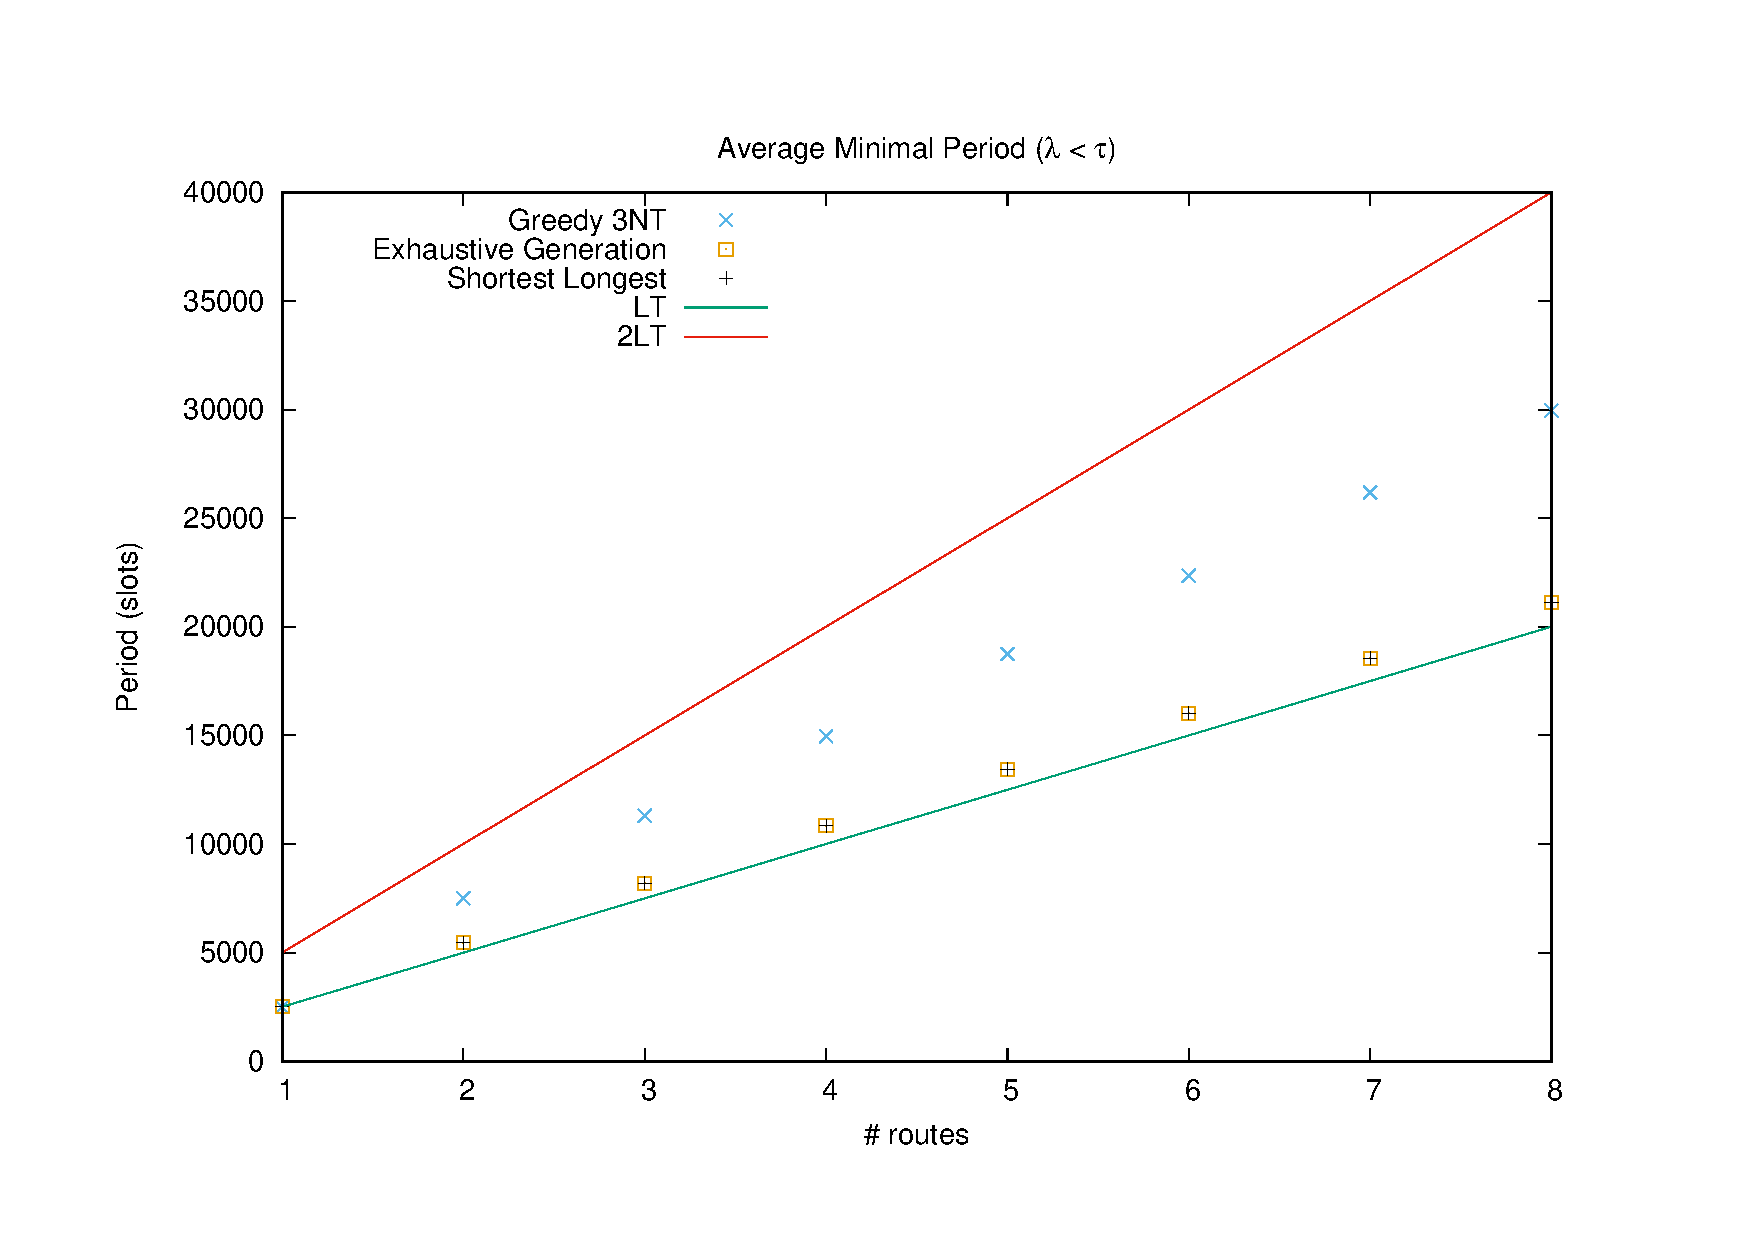
\includegraphics[scale=0.4]{periode_petite.pdf}
      \end{center}
     \caption{Minimum period found by the algorithms averaged over $1000$ random instances for each number of routes.}
\end{figure}
      
      First, we remark that the period found by the exhaustive search is only very slightly above the lower bound 
      $n\tau$, which means that, in this regime, it is very well justified to look for a solution without waiting time even for a highly loaded network. 
      
      The period needed by Shortest-Longest to find an optimal solution is determined by the difference between the longest and the shortest route and could be easily determined theoretically. The algorithm was expected to be good since the routes are short, but it turns out it always finds the optimal solution in our experiments. Therefore, we should use it in practical application, in this regime, instead of the exhaustive search which is much more computationally expensive. 
      
      Finally we remark that the greedy algorithm have an average period much lower than the theoretical upper bound of $3n\tau$. We made a linear regression on this value and with a correlation coefficient greater than $0,999$ we find a slope of $1.53n\tau$.
      
      

      \paragraph{Long routes}
      We now want to look at the performance of those algorithm if we significantly increase the size of the route. By increasing the size of the routes, the cuts of the exhaustive search, are less efficient. Thus, we defined a counter that allow the exhaustive search to end if no solutions are found.
      
      Since the exhaustive generation can fail, this is necessary to change the method to measure the minimum period for each algorithm, when the routes are long.      
      The following figure shows us the average success rate of the algorithms, on $1000$ instances, according to the period, with 8 routes, in which $\lambda(c_t,r_{t_i})$, are drawn following an uniform distribution between $0$ and $30000$ slots, that correspond to have the size of the route and the period approximately in the same range.
      
      The reason why the shortest longest were optimal in the previous experiences ,i.e. having a small difference between the longest and the shortest route, is no longer reviewed. In this situation, this difference can be considerable, and then the required period too.
      
      One the other hand, one can imagine that the greedy $3.n.\tau$ algorithm finds reasonable solutions, because the algorithm does not consider the size of the route, and thus, is not impacted by this parameter.
      
      On the following figure, the upper bound represents the cases in which the exhaustive search found a solution plus the number of {\em early} halts of the search. The real upper bound is probably between those two curves.
\begin{figure}

       \begin{center}
      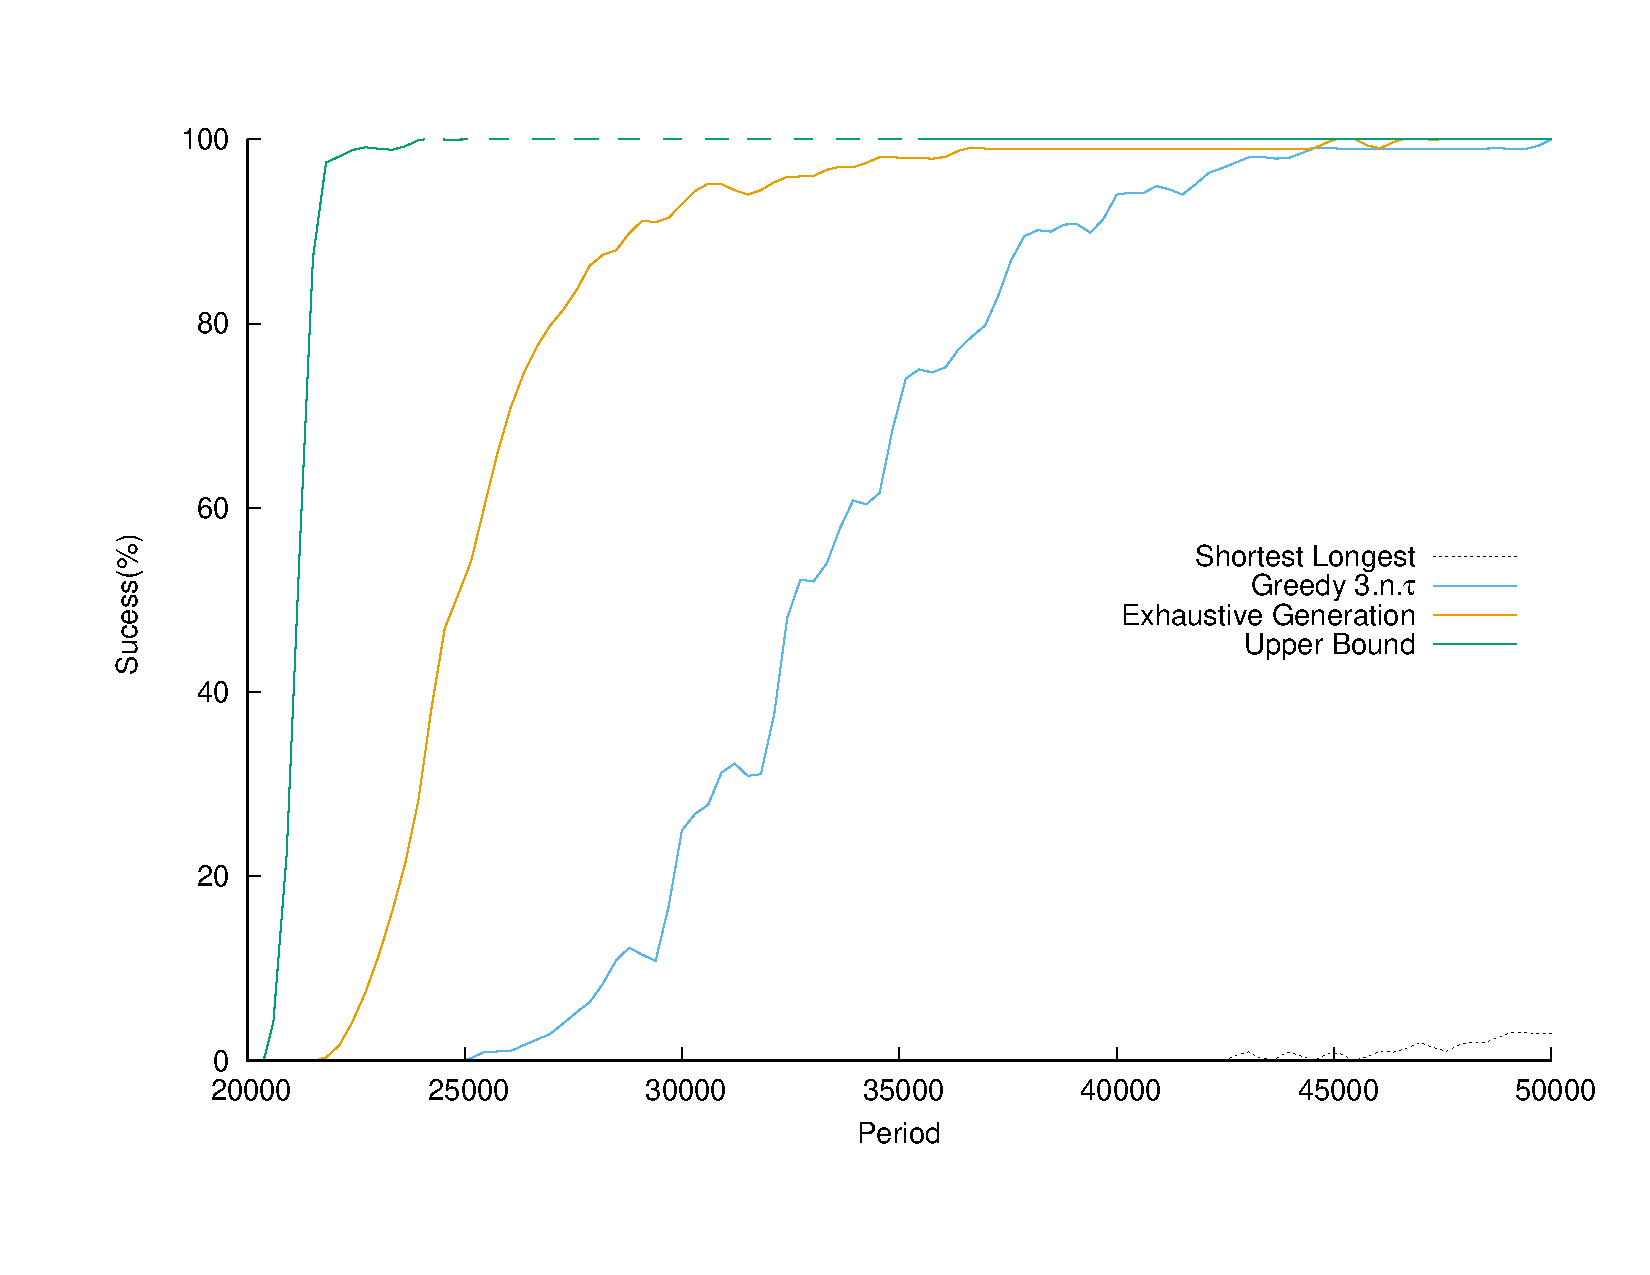
\includegraphics[scale=0.4]{echec_longues.pdf}
      \end{center}
      \caption{Success rate of the algorithms according to the period for long routes.}
     \end{figure}
      
      As we can see, Shortest longest has a very low success rate, and is not efficient anymore with those parameters.
      Whereas, the greedy algorithm gives us solutions with much lower period than Shortest Longest. The exhaustive search keeps finding good solutions in short periods but it fails a lot for periods that does not give a lot of flexibility in the backward period. This mean that, for a small period, a solution may exists, but the exhaustive search needs too much time to find it. In this situation, it could be better to use the greedy algorithm, that find a good solution in a polynomial time.

          
      So, those experiences shows us that, for C-RAN topologies, with small routes, shortest-longest finds some optimal affectations in a polynomial time, but, the longer the routes are, the better it is to use the greedy policy to find a solution without waiting times in a polynomial time.\\
    
      As we just saw, if the load increases, the needed period increases too, and it is not possible anymore to find a solution without waiting times with a small period. The next sections treats about the proposed solutions to find a $(P,\tau)$ periodic affectation when the period is small.
   \subsection{Allowing waiting times}
    
     \subsubsection{Intro}
     
	  In the previous section, we described some algorithm to solve an easier version of PALL, in which there is no waiting times. As we just conclude, this problem cannot be solved when the period is too small. The C-RAN context gives us a fixed period, thus, some topologies with a lot of routes might be impossible to schedule with the previous algorithms. We propose to allow some message to wait in the target vertices (BBU), with the aim of giving an higher degree of freedom for the scheduling. In this section, the waiting times $w_i$ are not necessarily null anymore. Thus, $MT({\cal M})$ might be superior to $T_{max}$ and it is necessary to minimize $MT({\cal M})$.
	   

% 
% 	

     \subsubsection{A first approach}
	  

      To find a solution with waiting times, the following heuristic is suggested:

      On the forward period, the messages are scheduled so that they are following each others, from the one using the longest route, to the one using the shortest route. Thus, we set the $m_{s_i}$ of the routes such that  $t(c_s,r_{s_i}) = \tau.i$, if the routes $r_i$ are ordered from the longest to the shortest.

      On $c_t$, the policy is the following one, after setting the clock to 0:
      \begin{enumerate}
      \item To be eligible, a message needs to be able to come back on $c_t$ at the current clock (if clock = 0, take the first message able to come back).
      \item Between the eligible messages, schedule first the one which has the lowest deadline.
      \item Repeat until all the messages had been scheduled.
      \end{enumerate}

      For any route i, the deadline correspond to $m_{s_i} + T_{max}-t(c_s,r_{s_i})$. This deadline corresponds to the latest date at which a message is able to quit the target switch without exceed $T_{max}$.
% 
% \begin{algorithm}[H]
% \caption{Longest Shortest Greedy (LSG)}
% \begin{algorithmic}
% \REQUIRE routage graph ${\cal R_{\cal C}}$, period $P$, packet size $\tau$
% \ENSURE $(P-\tau)-$periodic affectation of ${\cal R_{\cal C}}$
% \STATE clock $\leftarrow$ 0
% \FORALL{route i in $r_{s_i}$ from the longest to the shortest }
% \STATE  $m_{s_i} \leftarrow$ clock
% \STATE clock $\leftarrow$ clock + $\tau$
% \ENDFOR
% \STATE clock $\leftarrow$ 0
% \STATE take i such that $r_{\cal C(s_i)}$ is the first route to come back in sources switch
% \STATE $m_{\cal C(s_i)} \leftarrow $ clock;
% \STATE clock $\leftarrow$ $t(c_t,r_{\cal C(s_i)})$ + $\tau$
% \WHILE{there is a route which has not been scheduled}
% \STATE take i such that $r_{\cal C(s_i)}$ is the eligible route.
% \STATE $m_{\cal C(s_i)} \leftarrow $ clock - $t(c_t,r_{\cal C(s_i)})$;
% \STATE clock $\leftarrow$ clock + $\tau$
% 
% \ENDWHILE
% 
% \end{algorithmic}
% \end{algorithm}
\todo{ecrire l'algo}

	\paragraph{Particular case corresponding to C-RAN}
		
	One of the closest approach to real networks is the case in which all the weight on the arcs going from $c_t$ to targets are the, this algorithm gives an optimal solution. Indeed, all the same weight can be simplified by 0, thus the scheduling in the forward and backward period is the same, that is, all message following each others, so the period is minimal : $n.\tau$, where $n$ is the number of routes. Furthermore, all the waiting times are set to 0 i.e. $w_i = 0,\forall i \in n$, thus, $MT({\cal M})$ is equal to twice the longer delay of the routes, that is not alterable.

	\paragraph{Another particular case}
	Another case of this topology is the case in which all the weight on the arcs between $c_s$ and the sources are the same.
	In this case, the algorithm gives optimal solutions too:\\

	Since we can simplify the weight on the arcs between $c_s$ and the sources, we consider only the delay between $c_t$ and the targets. Order the routes such that $\lambda(r_{s_i}) > \lambda(r_{s_j}), i,j \in n, i<j$, i.e. the route 1 is the longest one, and the route $n$ is the shortest.
	The messages are sent in the forward period from 0 to $n-1$, that is $m_{s_i} = \tau * n$.
	The first message has totally reach the backward period at time $2.\lambda(r_{s_0})+\tau$. The process time of the first message is $PT(s_0) = 2.\lambda(r_{s_0}) $.
	The second message is eligible in the backward period at time $\tau + 2.\lambda(r_{s_1})$. Thus, the waiting time of the second route is $w_{s_1} = 2.\lambda(r_{s_0})+\tau - (\tau + 2.\lambda(r_{s_1})) = 2.(\lambda(r_{s_0}) - \lambda(r_{s_1}))$. Thus $PT(s_1) = 2.\lambda(r_{s_1}) + 2.(\lambda(r_{s_0}) - \lambda(r_{s_1}))  = 2.\lambda(r_{s_0})  = PT(s_0)$.
	By induction, $PT(s_i) = PT(s_0), \forall i \in n$. 
	Consequently, for this case, the heuristic is optimal, because the longest route has no waiting time all the other routes has the exact same process time, thus, $MT(M) = PT(s_0) = 2.\lambda(r_{s_0}) $.

	This results is available because we do not consider the weight on links before $c_s$.

     \subsubsection{Sending order}
	When then tried to look at the behaviour of the greedy policy with different kind of sending the messages, in the first way.
	
	We tried the five following sending policy, on the first way, and we applied the greedy heuristic to the way back, considering the offsets given by the sending policy used.
	The different sending policy are the following :
	\begin{enumerate}
	 \item trying $X$ random permutations of the routes, until one gives an available $(P,\tau)$ periodic affectation.
	 \item from the longest to the shortest route.
	 \item from the shortest to the longest route.
	 \item from the longest to the shortest arc between $c_t$ an the target.
	 \item from the shortest to the longest arc between $c_t$ an the target.
	\end{enumerate}


	\todo{Mettre les prametres d'une experience ou on voit le taux de réussite des différents départs}
     \subsubsection{A better Algorithm : periodicity}
     
     The previous algorithm is a greedy heuristic, which does not take the period into account. Thus, some given solution by this algorithm need a too large period an thus, are not available. 
     We propose an improved version of the algorithm, still greedy, but which consider the period.
     
     The greedy policy is the same, but
     
     \subsubsection{Another better Algorithm : $T_{MAX}$}
     
     \subsubsection{Mix : Simons periodic}
     
	
   
\section{Conclusion}



\bibliographystyle{ieeetr}
\bibliography{Sources.bib}

\end{document}
